% begin with an Alon-Fershtman slide; review as quicly as possible ``because many people here are familar with this paper, I'll try to keep this short'' Maybe check with david that this is a good idea
% Then jump into my key contribution: how do we think about the priors

%%%%%%%%%%%%%%%%%%%%%%%%%%%%%%%%%%%%%%%%%%%%%%%%%%%%%%%%%%%%%%%%%%%%%%%%%%%%%%%%
%%%%%%%%%%%%%%%%%%%%%%%%%%%%%%%%%%%%%%%%%%%%%%%%%%%%%%%%%%%%%%%%%%%%%%%%%%%%%%%%
\begin{frame}{Model preliminaries}

% Discrete time
% Infinitely lived agents

% unknown success probability in j

% write that with an indicator function

% 

Individuals endowed with:
\begin{itemize}
    \item [$h_{j0}$:] Skill-$j$ specific human capital ($j=0,\dots,J$)
    \item [$\theta_j$:] Unknown probability of success in $j$
    \item [$P_{j0}$:] Prior beliefs about $\theta_j$
\end{itemize}



\vspace{2ex}
Time constraint: At each $t$, individuals can choose to either study ($\study_{jt}$)
or work ($\ell_{jt}$) in one field $j \in \{1, \dots, J\}$:
\begin{equation*}
    \sum_{j=0}^J (\study_{jt} + \ell_{jt}) = 1, \quad \quad \study_{jt}, \ell_{jt} \in \{0, 1\}
\end{equation*}
\vspace{-2.5ex}
\begin{itemize}
    % \item $\study_{jt} = 1 \implies$ use time $t$ to study field $j$
    \item Studying may accumulates field-$j$ human capital and reveals information about underlying probability of success in $j$
    % \begin{itemize}
    %   \item [$\implies$] $m_{jt} = 1$
    % \end{itemize}
    % Endogenous enter labor market at time t as a skill j specialist to maximize 
    % \item $\ell_{jt} = 1 \implies $ use time $t$ to work in field $j$ 

    
    % \item Use time $t$ to study field $j$ $\implies \study_{jt} = 1$; otherwise $\study_{jt} = 0$
    % \begin{itemize}
    %   \item Accumulates field-$j$ human capital
    %   \item Reveals information about underlying prob. of success in $j$
    % \end{itemize}
    % \item Use time $t$ to work in field $j$ $\implies \ell_{jt} = 1$; otherwise $\ell_{jt} = 0$
    % \begin{itemize}
    %   \item Receive wage $w_j$
    % \end{itemize}
    \item If you work, you receive wage $w_j$
% To keep things simple, I'll assume utility is linear, and that the value of entering the market in period t as a skill k specialist simply depends on lifetime earnings
\end{itemize}


\vspace{2ex}
Enter labor market at time $t$ in skill-$j$ to maximize expected lifetime payoff:
\begin{equation*}
    \frac{\delta^t}{1 - \delta} U_j (w_{j}, h_{jt}) \ell_{jt}
    = \frac{\delta^t}{1 - \delta} w_{j} h_{jt} \ell_{jt}
    % Is it okay to say this? 
\end{equation*}
% \vspace{2ex}


\end{frame}

%%%%%%%%%%%%%%%%%%%%%%%%%%%%%%%%%%%%%%%%%%%%%%%%%%%%%%%%%%%%%%%%%%%%%%%%%%%%%%%%
% \begin{frame}{Student specialization decision}
\begin{frame}{Evolution of human capital accumulation and beliefs}

% Choose probability 

Students studying skill-$j$ at time $t$ pass the course with probability $\theta_j$:
\begin{equation*}
    \pass_{jt} \sim \text{Bernoulli} (\theta_j)
\end{equation*}
\vspace{-2.5ex}
\begin{itemize}
  \item 
  Accumulate human capital if they pass the course:
  \begin{align*}
  % h_{jt+1} =& H(h_{kt}, a_{kt}), \quad \quad
%   % a_{jt} \sim F_{\theta_j}
    h_{jt+1} = h_{jt} + \nu_{j} \pass_{jt} \study{jt}
  \end{align*}
  \item 
  Beliefs about $\theta_j$ evolve:
  \begin{equation*}
      \mgreen<2->{P_{j,t+1}} = \Pi_j (\mblue<2->{P_{jt}}, \pass_{jt})
        % P_{j, t+1} 
  \end{equation*}
\end{itemize}

\pause
\vspace{5ex}
\textbf{Key:} How are  \blue<2->{priors} formed, and how are they \green{updated}? 

% Parameter we are trying to understand is probability of success
% Know that we want a prior distribution supported on [0, 1]

\end{frame}

%%%%%%%%%%%%%%%%%%%%%%%%%%%%%%%%%%%%%%%%%%%%%%%%%%%%%%%%%%%%%%%%%%%%%%%%%%%%%%%%
\begin{frame}[t]{Belief distribution}

Initial prior drawn from Beta distribution 
\begin{equation*}
    \mblue{P_{j0}} = \mathcal{B} (\alpha_{j0}, \beta_{j0})
\end{equation*}
% Beta distribution is appropriate 
% need a probability distribution supported on [0,1]
% Also has some desireable analytic properties
Update according to Bayes Rule $\implies$ posterior drawn from Beta distribution:
\begin{equation*}
    \mgreen{P_{j,t+1}} = \mathcal{B} (\alpha_{j,t+1}, \beta_{j,t+1}), \quad \quad 
    (\alpha_{j,t+1}, \beta_{j,t+1}) = 
    \begin{cases} 
        (\alpha_{jt} + 1, \beta_{jt}) &\text{ if } a_{jt} = 1 \\
        (\alpha_{jt}, \beta_{jt} + 1) &\text{ if } a_{jt} = 0
    \end{cases}
\end{equation*}

\vspace{3ex}
\begin{columns}[T] % align columns
\begin{column}{.51\textwidth}

\pause
\vspace{3ex}
Example: $\alpha_0 = 1$, $\beta_0 = 1$
\vspace{1.5ex}
\begin{itemize}
    \item <3-> success at $t=1$ $\implies$ $\alpha_1 = 2$, $\beta_1 = 1$

    \vspace{1.5ex}
    \item <4-> failure at $t=2$ $\implies$ $\alpha_1 = 2$, $\beta_1 = 2$
    
    \vspace{1.5ex}
    \item <5-> success at $t=3$ $\implies$ $\alpha_1 = 3$, $\beta_1 = 2$
\end{itemize}

\end{column}%
% \hfill%
\begin{column}{.39\textwidth}
\begin{figure}
\only<2>{% This file was created by tikzplotlib v0.9.1.
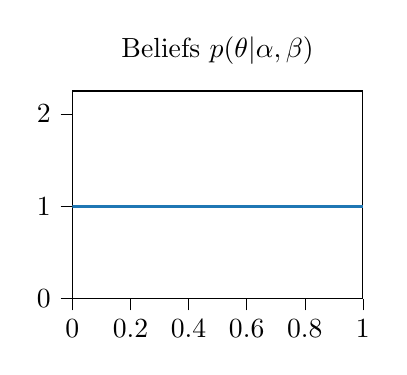
\begin{tikzpicture}

\definecolor{color0}{rgb}{0.12156862745098,0.466666666666667,0.705882352941177}

\begin{axis}[
height=120pt,
tick align=outside,
tick pos=left,
title={Beliefs \(\displaystyle p(\theta | \alpha, \beta)\)},
width=150pt,
x grid style={white!69.0196078431373!black},
xmin=0, xmax=1,
xtick style={color=black},
y grid style={white!69.0196078431373!black},
ymin=0, ymax=2.25,
ytick style={color=black}
]
\addplot [very thick, color0]
table {%
0 1
1 1
};
\end{axis}

\end{tikzpicture}
}
\only<3>{% This file was created by tikzplotlib v0.9.1.
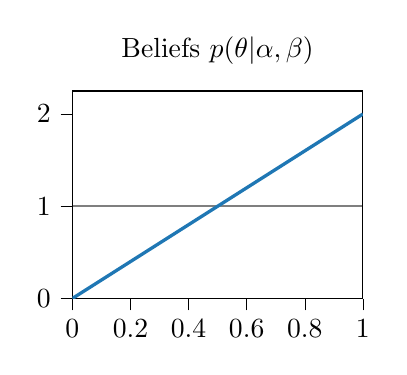
\begin{tikzpicture}

\definecolor{color0}{rgb}{0.12156862745098,0.466666666666667,0.705882352941177}

\begin{axis}[
height=120pt,
tick align=outside,
tick pos=left,
title={Beliefs \(\displaystyle p(\theta | \alpha, \beta)\)},
width=150pt,
x grid style={white!69.0196078431373!black},
xmin=0, xmax=1,
xtick style={color=black},
y grid style={white!69.0196078431373!black},
ymin=0, ymax=2.25,
ytick style={color=black}
]
\addplot [semithick, black, opacity=0.5]
table {%
0 1
1 1
};
\addplot [very thick, color0]
table {%
0 0
1 2
};
\end{axis}

\end{tikzpicture}
}
\only<4>{% This file was created by tikzplotlib v0.9.2.
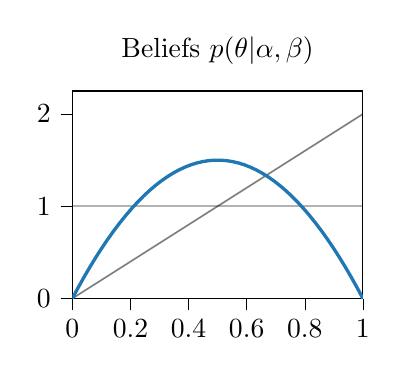
\begin{tikzpicture}

\definecolor{color0}{rgb}{0.12156862745098,0.466666666666667,0.705882352941177}

\begin{axis}[
height=120pt,
tick align=outside,
tick pos=left,
title={Beliefs \(\displaystyle p(\theta | \alpha, \beta)\)},
width=150pt,
x grid style={white!69.0196078431373!black},
xmin=0, xmax=1,
xtick style={color=black},
y grid style={white!69.0196078431373!black},
ymin=0, ymax=2.25,
ytick style={color=black}
]
\addplot [semithick, black, opacity=0.3]
table {%
0 1
1 1
};
\addplot [semithick, black, opacity=0.5]
table {%
0 0
1 2
};
\addplot [very thick, color0]
table {%
0 0
0.0204081535339355 0.11995005607605
0.0408163070678711 0.234902143478394
0.0612244606018066 0.344856262207031
0.0816326141357422 0.449812650680542
0.102040767669678 0.549770951271057
0.122448921203613 0.644731283187866
0.142857193946838 0.734693884849548
0.163265347480774 0.819658517837524
0.183673501014709 0.899625182151794
0.204081654548645 0.974593877792358
0.224489808082581 1.04456472396851
0.244897961616516 1.10953772068024
0.265306115150452 1.16951274871826
0.285714268684387 1.22448980808258
0.306122422218323 1.27446901798248
0.326530575752258 1.31945025920868
0.346938848495483 1.35943353176117
0.367347002029419 1.39441895484924
0.387755155563354 1.4244065284729
0.40816330909729 1.44939613342285
0.428571462631226 1.4693877696991
0.448979616165161 1.48438155651093
0.469387769699097 1.49437737464905
0.489795923233032 1.49937522411346
0.510204076766968 1.49937522411346
0.530612230300903 1.49437737464905
0.551020383834839 1.48438155651093
0.571428537368774 1.4693877696991
0.59183669090271 1.44939613342285
0.612244844436646 1.4244065284729
0.632652997970581 1.39441895484924
0.653061151504517 1.35943353176117
0.673469305038452 1.31945025920868
0.693877577781677 1.27446901798248
0.714285731315613 1.22448980808258
0.734693884849548 1.16951274871826
0.755102038383484 1.10953772068024
0.775510191917419 1.04456472396851
0.795918345451355 0.974593877792358
0.81632661819458 0.899625182151794
0.836734771728516 0.819658517837524
0.857142925262451 0.734693884849548
0.877551078796387 0.644731283187866
0.897959232330322 0.549770951271057
0.918367385864258 0.449812650680542
0.938775539398193 0.344856262207031
0.959183692932129 0.234902143478394
0.979591846466064 0.11995005607605
1 0
};
\end{axis}

\end{tikzpicture}
}
\only<5>{% This file was created by tikzplotlib v0.9.2.
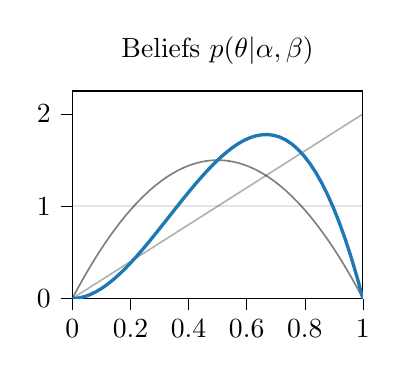
\begin{tikzpicture}

\definecolor{color0}{rgb}{0.12156862745098,0.466666666666667,0.705882352941177}

\begin{axis}[
height=120pt,
tick align=outside,
tick pos=left,
title={Beliefs \(\displaystyle p(\theta | \alpha, \beta)\)},
width=150pt,
x grid style={white!69.0196078431373!black},
xmin=0, xmax=1,
xtick style={color=black},
y grid style={white!69.0196078431373!black},
ymin=0, ymax=2.25,
ytick style={color=black}
]
\addplot [semithick, black, opacity=0.1]
table {%
0 1
1 1
};
\addplot [semithick, black, opacity=0.3]
table {%
0 0
1 2
};
\addplot [semithick, black, opacity=0.5]
table {%
0 0
0.0204081535339355 0.11995005607605
0.0408163070678711 0.234902143478394
0.0612244606018066 0.344856262207031
0.0816326141357422 0.449812650680542
0.102040767669678 0.549770951271057
0.122448921203613 0.644731283187866
0.142857193946838 0.734693884849548
0.163265347480774 0.819658517837524
0.183673501014709 0.899625182151794
0.204081654548645 0.974593877792358
0.224489808082581 1.04456472396851
0.244897961616516 1.10953772068024
0.265306115150452 1.16951274871826
0.285714268684387 1.22448980808258
0.306122422218323 1.27446901798248
0.326530575752258 1.31945025920868
0.346938848495483 1.35943353176117
0.367347002029419 1.39441895484924
0.387755155563354 1.4244065284729
0.40816330909729 1.44939613342285
0.428571462631226 1.4693877696991
0.448979616165161 1.48438155651093
0.469387769699097 1.49437737464905
0.489795923233032 1.49937522411346
0.510204076766968 1.49937522411346
0.530612230300903 1.49437737464905
0.551020383834839 1.48438155651093
0.571428537368774 1.4693877696991
0.59183669090271 1.44939613342285
0.612244844436646 1.4244065284729
0.632652997970581 1.39441895484924
0.653061151504517 1.35943353176117
0.673469305038452 1.31945025920868
0.693877577781677 1.27446901798248
0.714285731315613 1.22448980808258
0.734693884849548 1.16951274871826
0.755102038383484 1.10953772068024
0.775510191917419 1.04456472396851
0.795918345451355 0.974593877792358
0.81632661819458 0.899625182151794
0.836734771728516 0.819658517837524
0.857142925262451 0.734693884849548
0.877551078796387 0.644731283187866
0.897959232330322 0.549770951271057
0.918367385864258 0.449812650680542
0.938775539398193 0.344856262207031
0.959183692932129 0.234902143478394
0.979591846466064 0.11995005607605
1 0
};
\addplot [very thick, color0]
table {%
0 0
0.0204081535339355 0.00489592552185059
0.0408163070678711 0.01917564868927
0.0612244606018066 0.0422272682189941
0.0816326141357422 0.0734387636184692
0.102040767669678 0.112198114395142
0.122448921203613 0.157893419265747
0.142857193946838 0.209912538528442
0.163265347480774 0.267643570899963
0.183673501014709 0.330474615097046
0.204081654548645 0.397793412208557
0.224489808082581 0.468988299369812
0.244897961616516 0.543447017669678
0.265306115150452 0.62055778503418
0.285714268684387 0.699708461761475
0.326530575752258 0.861681699752808
0.367347002029419 1.02447104454041
0.387755155563354 1.10464179515839
0.40816330909729 1.18318045139313
0.428571462631226 1.25947523117065
0.448979616165161 1.33291399478912
0.469387769699097 1.40288484096527
0.489795923233032 1.46877574920654
0.510204076766968 1.52997469902039
0.530612230300903 1.58586978912354
0.551020383834839 1.63584899902344
0.571428537368774 1.67930030822754
0.59183669090271 1.71561169624329
0.612244844436646 1.74417126178741
0.632652997970581 1.76436686515808
0.653061151504517 1.77558672428131
0.673469305038452 1.77721869945526
0.693877577781677 1.76865077018738
0.714285731315613 1.74927115440369
0.734693884849548 1.71846759319305
0.755102038383484 1.67562830448151
0.775510191917419 1.62014126777649
0.795918345451355 1.55139434337616
0.81632661819458 1.46877574920654
0.836734771728516 1.3716733455658
0.857142925262451 1.25947523117065
0.877551078796387 1.13156938552856
0.897959232330322 0.987343788146973
0.918367385864258 0.826186418533325
0.938775539398193 0.647485256195068
0.959183692932129 0.450628519058228
0.979591846466064 0.235004186630249
1 0
};
\end{axis}

\end{tikzpicture}
}
\end{figure}
\end{column}%
\end{columns}
% \hypertarget<2>{beta_11_example}{\beamerbutton{I'm on the fourth slide}}
\hypertarget<2>{model_beta_11}{
  \hyperlink{simulate}{\beamerbutton{Return: simulation set-up}}
  \hyperlink{sim_default}{\beamerbutton{Return: baseline simulation}}
}
\hypertarget<4>{model_beta_22}{\hyperlink{sim_beliefs}{\beamerbutton{Return: simulation}}}
% \hyperlink{belief_effect}{\beamerbutton{Return: simulation}}


\end{frame}




%%%%%%%%%%%%%%%%%%%%%%%%%%%%%%%%%%%%%%%%%%%%%%%%%%%%%%%%%%%%%%%%%%%%%%%%%%%%%%%%
\begin{frame}{Group-based parametrization}



Consider group-based beliefs about abilities:
\begin{itemize}
    \item Each individual has a group type: $g \in \{m, f\}$

    \item Students form beliefs, $P_{j0}$, based on previously observed group successes
\end{itemize}

\vspace{2ex}
Simple parameterization:
\begin{itemize}
    \item [$\alpha_{j0}^g$: ] Number of type-$g$ students who have succeeded in $j$ 
    \item [$\beta_{j0}^g$: ] Number of type-$g$ students who have failed in $j$

    \item [$\implies$] Observed success rate:
    \begin{equation*}
    \mu_{j0}^g = 
      \frac{\alpha_{j0}^g}{\alpha_{j0}^g + \beta_{j0}^g}.
\end{equation*}
This average is based on a sample size of type $g$ students:
\begin{equation*}
    n_{j0}^g = \alpha_{j0}^g + \beta_{j0}^g
 \end{equation*}
\end{itemize}

\vspace{2ex}
Group-based prior beliefs about probability of success in skill-$j$ courses, $\theta_j$:
\begin{equation*}
    \mathcal{B} \pr{\alpha_{j0}^g, \beta_{j0}^g} \quad \implies \quad
    \mathcal{B} \pr{\mu_{j0}^g n_{j0}^g, (1 - \mu_{j0}^g) n_{j0}^g}
\end{equation*}



\end{frame}

%%%%%%%%%%%%%%%%%%%%%%%%%%%%%%%%%%%%%%%%%%%%%%%%%%%%%%%%%%%%%%%%%%%%%%%%%%%%%%%%
\begin{frame}{Group-based belief distribution}

% Suppose sample size of men is larger than that of women, but the observed success rate is the same for the two groups:
Suppose there are more men then women in field $j$: 
\begin{equation*}
  n_{j0}^m > n_{j0}^f
\end{equation*}
But the observed success rate is the same for the two groups:
\begin{equation*}
    \mu_{j0} = \mu_{j0}^m = \mu_{j0}^w
\end{equation*}

\begin{figure}
% This file was created by tikzplotlib v0.9.2.
\begin{tikzpicture}

\definecolor{color0}{rgb}{0.266666666666667,0.466666666666667,0.666666666666667}
\definecolor{color1}{rgb}{0.933333333333333,0.4,0.466666666666667}

\begin{axis}[
height=6.376357092455836cm,
legend cell align={left},
legend style={fill opacity=0.8, draw opacity=1, text opacity=1, at={(0.03,0.97)}, anchor=north west, draw=none},
tick align=outside,
tick pos=left,
width=10.317162499999998cm,
x grid style={white!69.0196078431373!black},
xmin=-0.05, xmax=1.05,
xtick style={color=black},
y grid style={white!69.0196078431373!black},
ymin=0, ymax=2.66141549653429,
ytick style={color=black}
]
\addplot [semithick, color0]
table {%
0 0
0.0580580234527588 0.000277876853942871
0.0750750303268433 0.000951051712036133
0.0880880355834961 0.00202715396881104
0.0990991592407227 0.00352215766906738
0.108108162879944 0.0052802562713623
0.117117166519165 0.00764262676239014
0.125125169754028 0.0103511810302734
0.132132172584534 0.0132688283920288
0.139139175415039 0.0167677402496338
0.146146178245544 0.0209178924560547
0.15315318107605 0.0257914066314697
0.160160183906555 0.0314624309539795
0.166166186332703 0.0370153188705444
0.17217218875885 0.0432579517364502
0.178178191184998 0.0502384901046753
0.184184193611145 0.0580054521560669
0.190190196037292 0.0666069984436035
0.19619619846344 0.0760910511016846
0.203203201293945 0.0883336067199707
0.210210204124451 0.101914048194885
0.217217206954956 0.116902947425842
0.224224209785461 0.133368015289307
0.231231212615967 0.151373624801636
0.238238215446472 0.170979976654053
0.245245218276978 0.192243218421936
0.252252221107483 0.215214252471924
0.260260224342346 0.243616461753845
0.268268227577209 0.274367570877075
0.276276350021362 0.307515382766724
0.284284353256226 0.343096613883972
0.292292356491089 0.381135225296021
0.301301240921021 0.426879644393921
0.310310363769531 0.475743412971497
0.319319248199463 0.527699708938599
0.329329371452332 0.588993549346924
0.339339375495911 0.65393853187561
0.350350379943848 0.729425430297852
0.361361384391785 0.808918356895447
0.37337338924408 0.899857521057129
0.386386394500732 1.00282371044159
0.401401400566101 1.12650215625763
0.419419407844543 1.28014957904816
0.448448419570923 1.53373908996582
0.473473429679871 1.75053000450134
0.489489555358887 1.88434946537018
0.50250244140625 1.98835706710815
0.513513565063477 2.07205963134766
0.523523569107056 2.14405512809753
0.532532453536987 2.2050347328186
0.541541576385498 2.2619833946228
0.549549579620361 2.30890417098999
0.556556582450867 2.34688472747803
0.563563585281372 2.38181519508362
0.56956958770752 2.40920257568359
0.575575590133667 2.43412804603577
0.581581592559814 2.45649647712708
0.586586594581604 2.47311806678772
0.591591596603394 2.48785185813904
0.596596598625183 2.50065088272095
0.600600600242615 2.50946736335754
0.604604601860046 2.51699638366699
0.608608603477478 2.52321815490723
0.611611604690552 2.527015209198
0.614614605903625 2.53005909919739
0.617617607116699 2.53234314918518
0.620620608329773 2.53386044502258
0.623623609542847 2.53460574150085
0.62662661075592 2.53457283973694
0.629629611968994 2.53375744819641
0.632632613182068 2.53215456008911
0.635635614395142 2.52976059913635
0.638638615608215 2.52657175064087
0.641641616821289 2.52258539199829
0.644644618034363 2.51779890060425
0.648648619651794 2.51016926765442
0.652652740478516 2.50111126899719
0.656656742095947 2.49062418937683
0.660660743713379 2.47870826721191
0.665665626525879 2.46180844306946
0.670670747756958 2.44268989562988
0.675675630569458 2.42136645317078
0.681681632995605 2.39289450645447
0.687687635421753 2.36131596565247
0.6936936378479 2.32668232917786
0.700700759887695 2.28249788284302
0.707707643508911 2.23435544967651
0.714714765548706 2.18238949775696
0.722722768783569 2.11851692199707
0.730730772018433 2.05011296272278
0.739739656448364 1.9681077003479
0.749749660491943 1.87126696109772
0.76076078414917 1.75860500335693
0.772772789001465 1.62956130504608
0.787787795066833 1.46146321296692
0.810810804367065 1.19596135616302
0.834834814071655 0.920849561691284
0.848848819732666 0.767037749290466
0.859859943389893 0.652013540267944
0.869869947433472 0.553140640258789
0.878878831863403 0.469607830047607
0.886886835098267 0.400230884552002
0.89489483833313 0.335862994194031
0.901901960372925 0.283928394317627
0.908908843994141 0.236297965049744
0.914914846420288 0.199018955230713
0.920920848846436 0.165092349052429
0.926926851272583 0.134564399719238
0.931931972503662 0.111733078956604
0.936936855316162 0.0912656784057617
0.941941976547241 0.0731372833251953
0.946946859359741 0.0573046207427979
0.950950980186462 0.0462501049041748
0.954954981803894 0.0365835428237915
0.958958983421326 0.0282543897628784
0.962962985038757 0.021202564239502
0.966966986656189 0.0153579711914062
0.970970988273621 0.0106403827667236
0.974974989891052 0.00695860385894775
0.978978991508484 0.00420975685119629
0.982982993125916 0.00227940082550049
0.986986994743347 0.00104022026062012
0.990990996360779 0.000352263450622559
0.996996998786926 1.34706497192383e-05
1 0
};
\addlegendentry{Men \\ ($\mu = $0.6, $n = $10)}
\addplot [semithick, color1]
table {%
0 0
0.00500500202178955 0.00029909610748291
0.0100100040435791 0.0011904239654541
0.0150150060653687 0.00266480445861816
0.0200200080871582 0.00471329689025879
0.0250250101089478 0.00732696056365967
0.0310310125350952 0.011196494102478
0.0370370149612427 0.0158512592315674
0.0430430173873901 0.021275520324707
0.0490490198135376 0.0274536609649658
0.0550550222396851 0.0343701839447021
0.0620620250701904 0.0433518886566162
0.0690690279006958 0.0532925128936768
0.0760760307312012 0.0641672611236572
0.0840840339660645 0.0777077674865723
0.0920920372009277 0.0923991203308105
0.101101160049438 0.110256433486938
0.11011016368866 0.129470825195312
0.119119167327881 0.149989724159241
0.12912917137146 0.174254298210144
0.139139175415039 0.199992060661316
0.150150179862976 0.229919075965881
0.161161184310913 0.261445164680481
0.173173189163208 0.297548055648804
0.186186194419861 0.338533163070679
0.200200200080872 0.384672880172729
0.21521520614624 0.436192035675049
0.231231212615967 0.493253231048584
0.249249219894409 0.559686422348022
0.269269227981567 0.635787844657898
0.293293237686157 0.729499101638794
0.327327370643616 0.864867448806763
0.379379391670227 1.07190155982971
0.403403401374817 1.16504085063934
0.423423409461975 1.24047493934631
0.441441416740417 1.30615937709808
0.457457423210144 1.36243712902069
0.472472429275513 1.41312110424042
0.486486434936523 1.45839333534241
0.499499559402466 1.49849700927734
0.511511564254761 1.5337210893631
0.522522449493408 1.56438684463501
0.533533573150635 1.59340107440948
0.543543577194214 1.61826372146606
0.553553581237793 1.64160966873169
0.562562584877014 1.66126477718353
0.571571588516235 1.67958033084869
0.580580592155457 1.69650363922119
0.58858859539032 1.71033525466919
0.596596598625183 1.72298836708069
0.603603601455688 1.73306393623352
0.610610604286194 1.74218416213989
0.617617607116699 1.75032413005829
0.623623609542847 1.75650227069855
0.629629611968994 1.76192653179169
0.635635614395142 1.76658129692078
0.641641616821289 1.77045083045959
0.646646618843079 1.773064494133
0.651651620864868 1.77511298656464
0.656656742095947 1.7765873670578
0.661661624908447 1.77747869491577
0.666666746139526 1.77777779102325
0.671671628952026 1.77747571468353
0.676676750183105 1.77656328678131
0.681681632995605 1.77503180503845
0.686686754226685 1.77287185192108
0.691691637039185 1.77007472515106
0.696696758270264 1.76663112640381
0.701701641082764 1.76253223419189
0.706706762313843 1.75776898860931
0.71271276473999 1.75116336345673
0.718718767166138 1.743572473526
0.724724769592285 1.73498058319092
0.730730772018433 1.72537219524384
0.73673677444458 1.71473157405853
0.742742776870728 1.70304334163666
0.749749660491943 1.68806207180023
0.756756782531738 1.67160880565643
0.763763785362244 1.65365862846375
0.770770788192749 1.63418686389923
0.777777791023254 1.61316871643066
0.785785794258118 1.58722269535065
0.793793797492981 1.55918765068054
0.801801800727844 1.5290265083313
0.809809803962708 1.49670231342316
0.817817807197571 1.46217811107635
0.826826810836792 1.42066276073456
0.835835814476013 1.37626349925995
0.844844818115234 1.32892775535583
0.853853940963745 1.27860295772552
0.862862825393677 1.22523641586304
0.872872829437256 1.16230869293213
0.882882833480835 1.09548842906952
0.892892837524414 1.02470362186432
0.902902841567993 0.949881792068481
0.912912845611572 0.870950937271118
0.923923969268799 0.779294729232788
0.934934854507446 0.682483077049255
0.945945978164673 0.580419778823853
0.95695698261261 0.473008632659912
0.967967987060547 0.360153555870056
0.978978991508484 0.241758584976196
0.990990996360779 0.106168985366821
1 0
};
\addlegendentry{Women \\ ($\mu = $0.6, $n = $5)}
\addplot [semithick, white!73.3333333333333!black, dotted, forget plot]
table {%
0.600000023841858 0
0.600000023841858 2.66141557693481
};
\end{axis}

\end{tikzpicture}

\end{figure}


\end{frame}


%%%%%%%%%%%%%%%%%%%%%%%%%%%%%%%%%%%%%%%%%%%%%%%%%%%%%%%%%%%%%%%%%%%%%%%%%%%%%%%%

% \nts{Frame remaining simple parameterization}
\begin{frame}{Individual problem}


A policy $\pi: (h_t, P_t^g) \to (s_t, \ell_t)$ is optimal if it maximizes:
\begin{align*}
& \mathbb{E}^\pi \sbr{
   \sum_{t=0}^\infty \delta^t 
   \left. \pr{\sum_{j=1}^J h_{jt} w_j \ell_{jt} } \right\vert
   \pr{(h_{10}, P_{10}^g), \dots, (h_{J0}, P_{J0}^g)}
} 
\end{align*}
Subject to the human capital accumulation and belief transition laws:
\begin{align*}
    h_{jt+1}^{} =& h_{jt}^{} + \nu_j \pass_{jt}^{}  \study_{jt}^{}, 
    \quad \quad 
    \pass_{jt}^{} \sim \text{Bernoulli} (\theta_j), 
    \quad \quad
    \theta_{j} \sim P_{j0}^{g} \equiv \mathcal{B} (\alpha_{j0}^g, \beta_{j0}^g),
    \\
    P_{j,t+1}^g =& \mathcal{B} (\alpha_{j,t+1}^g, \beta_{j,t+1}^g), 
    \quad \quad 
    (\alpha_{j,t+1}^{g}, \beta_{j,t+1}^{g}) = 
    \begin{cases} 
        (\alpha_{jt}^g + 1, \beta_{jt}^g) &\text{ if } \study_{jt}^g = 1 \text{ and } \pass_{jt}^g = 1 \\
        (\alpha_{jt}^g, \beta_{jt}^g + 1) &\text{ if } \study_{jt}^g = 1 \text{ and } \pass_{jt}^g = 0 \\
        (\alpha_{jt}^g, \beta_{jt}^g) &\text{ if } \study_{jt}^g = 0
    \end{cases}
    .
\end{align*}
And subject to the constraints:
\begin{align*}
&\sum_{j=1}^J (\study_{jt} + \ell_{jt}) = 1, \quad \quad \study_{jt}, \ell_{jt} \in \{0,1\} \\
&h_{j0} \leq \nu_j \alpha_{j0}^{g}
\end{align*}

\end{frame}

%%%%%%%%%%%%%%%%%%%%%%%%%%%%%%%%%%%%%%%%%%%%%%%%%%%%%%%%%%%%%%%%%%%%%%%%%%%%%%%%
\begin{frame}{Optimal policy rule}

Define the skill $j$ index as the expected payoff if you committed to studying $j$:
%\gen{ 
\begin{equation*}
\mathcal{I}_{jt} (h_{j}^g, P_{j}^g) = \sup_{\tau \geq 0} \mathbb{E}^\tau
\ce{
   \sum_{t=0}^\infty \delta^t 
   U_j(h_{jt}^g, w_j) \ell_{jt}^g
}{
    (h_{j0}^g, P_{j0}^g) = (h_{j}^g, P_{j}^g)
}
\end{equation*}

Define the graduation region of skill $j$ as: 
\begin{equation*}
\mathcal{G}_j (h_{j}^g, P_{j}^g)  = 
    \left\{
        (h_{j}^g, P_{j}^g) 
        \left\vert
            \arg \max_{\tau \geq 0} 
            \mathbb{E}^\tau 
            \ce{
                \sum_{t=0}^\infty \delta^t 
                U_j(h_{jt}^g, w_j) \ell_{jt}^g
            }{
                (h_j, P_j^g)
            } = 0
   \right. \right\}
\end{equation*}

The following policy $\pi: (h_t, P_t^g) \to (s_t, \ell_t)$ is optimal: 
\begin{enumerate}
    \item At each $t \geq 0$, choose skill $j^* = \arg \max_{j \in J} \mathcal{I}_j$, breaking ties according to any rule
    \item If $(h_{j^*}, P_{j^*}^g) \in \mathcal{G}_{j}$, then enter the labor market as a $j^*$ specialist. Otherwise, study $j^*$ for an additional period.  
\end{enumerate}

\end{frame}

%%%%%%%%%%%%%%%%%%%%%%%%%%%%%%%%%%%%%%%%%%%%%%%%%%%%%%%%%%%%%%%%%%%%%%%%%%%%%%%%

%%%%%%%%%%%%%%%%%%%%%%%%%%%%%%%%%%%%%%%%%%%%%%%%%%%%%%%%%%%%%%%%%%%%%%%%%%%%%%%

